\section{Results}\label{sec:results}

We apply our method to a set of mock data, the spherical models
for the Gaia challenge by Walker and Penarrubia. They consist of
dynamical tracer populations with density distribution

\begin{equation}
\nu_*(r) = \nu_0\left(\frac{r}{r_*}\right)^{-\gamma_*} \left[1+\left(\frac{r}{r_*}\right)^{\alpha_*}\right]^{(\gamma_*-\beta_*)/\alpha_*}
\end{equation}

inside dark matter halos of the form

\begin{equation}
\rho_{\text{DM}} = \rho_0\left(\frac{r}{r_{\text{DM}}}\right)^{-\gamma_{\text{DM}}}\left[1+\left(\frac{r}{r_{\text{DM}}}\right)^{\alpha_{\text{DM}}}\right]^{(\gamma_{\text{DM}}-\beta_{\text{DM}})/\alpha_{\text{DM}}}
\end{equation}

with scale radii $r_*, r_\text{DM}$, inner and outer logarithmic
slopes of $\gamma_*, \gamma_{\text{DM}}$ and
$\beta_*,\beta_{\text{DM}}$, with transition parameters $\alpha_*,
\alpha_{\text{DM}}$.

The anisotropy follows the functional form of \citet{Osipkov1979} and
\citet{Merritt1985},

\begin{equation}
\beta_{\text{anisotropy}}(r)=1-\frac{\sigma_\theta^2}{\sigma_r^2} = \frac{r^2}{r^2+r_a^2}.
\end{equation}

with scale radius $r_a$, turning over from nearly isotropic at $r\to
0$ to radially biased at $r_*=r_a$.

Of these distributions, finite samplings are taken and converted to
mock observational data including observational parameters like
spectral indices, systemic velocities, proper motions, and binary
motion.


\subsection{Cusps and Cores}

Applied on a profile with a core in the DM density profile, our method
reproduces the density profile \TODO{(fig. \ref{fig:cusp})}.

\begin{figure*}
\begin{center}
\hspace{-7mm}
%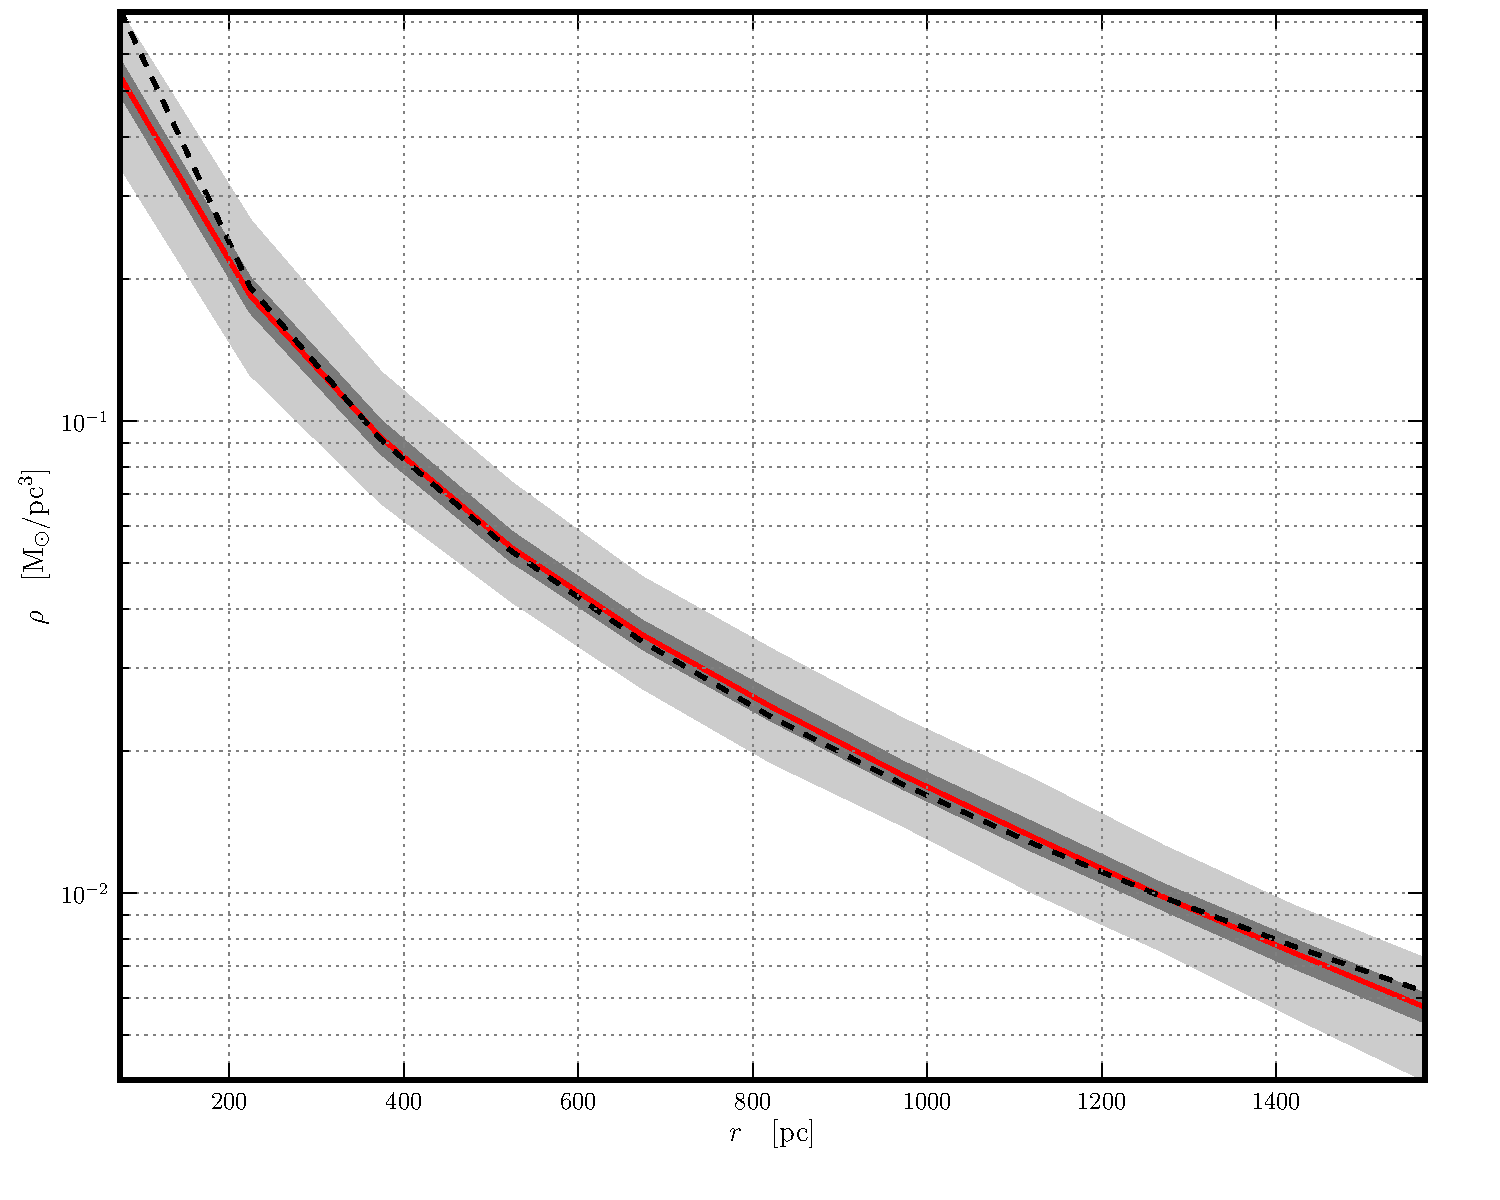
\includegraphics[width=0.5\textwidth]{fig/20130718132442_case_2_10000_0_cprior_nulog_denslog_mslope_rprior_profdens.pdf}
%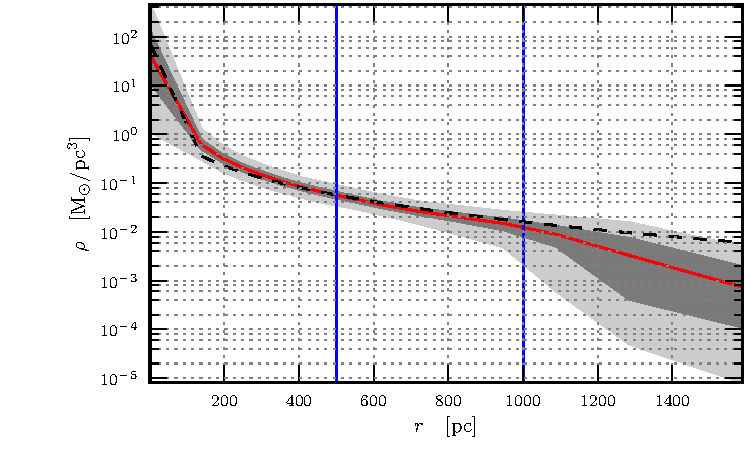
\includegraphics[width=0.5\textwidth]{fig/profdens.pdf}
%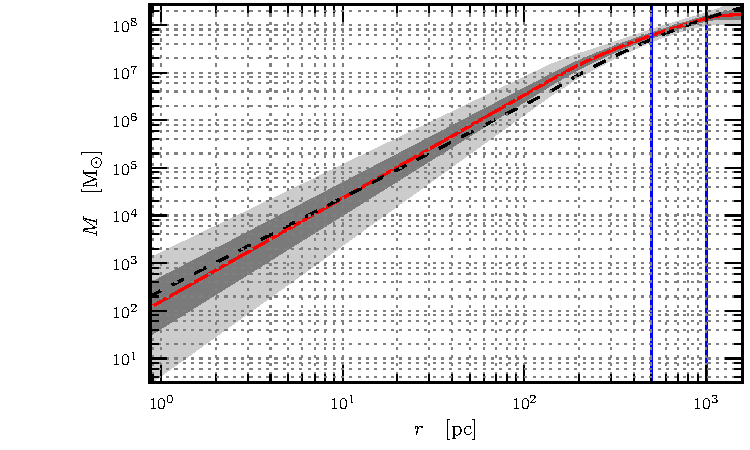
\includegraphics[width=0.5\textwidth]{fig/profM.pdf}
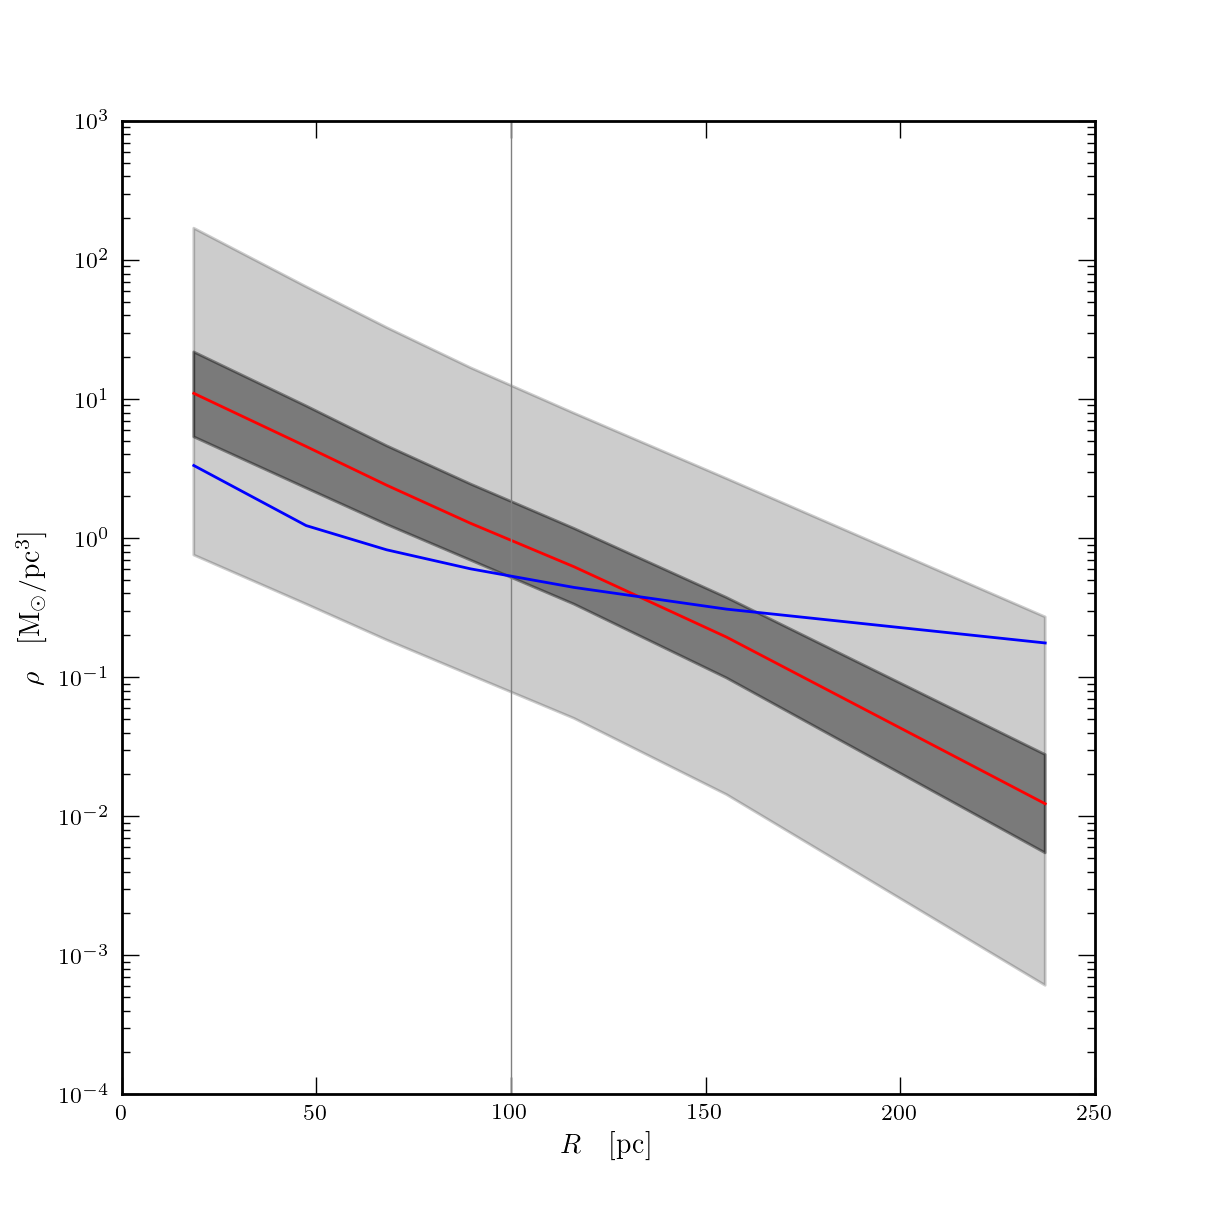
\includegraphics[width=0.3\textwidth]{fig/prof_dens.png}
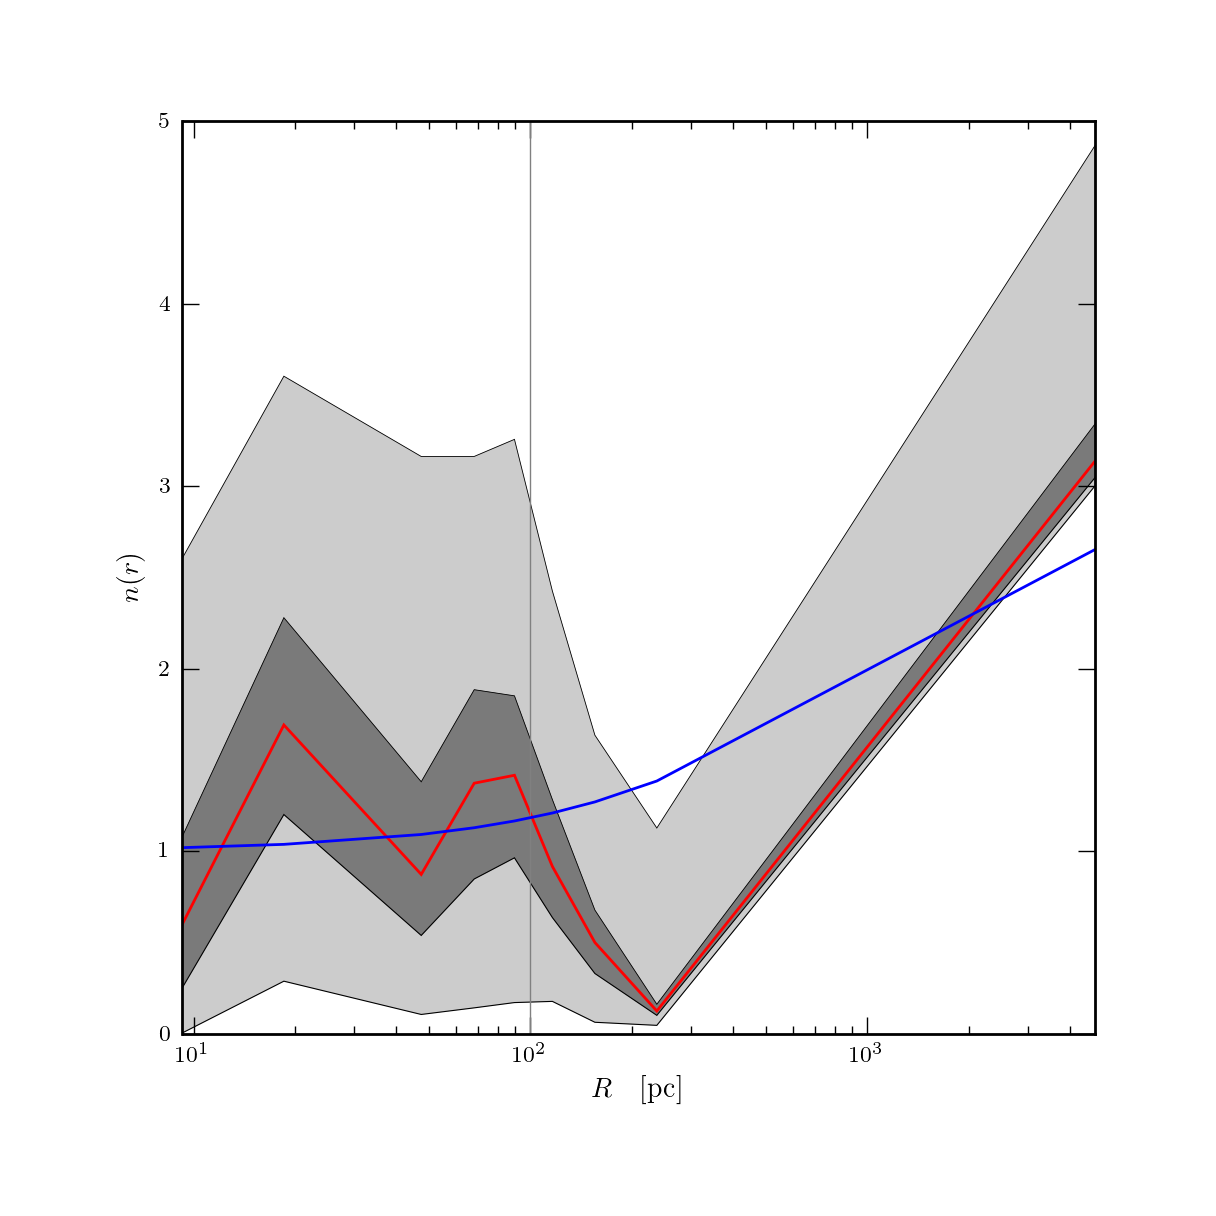
\includegraphics[width=0.3\textwidth]{fig/prof_nr.png}
%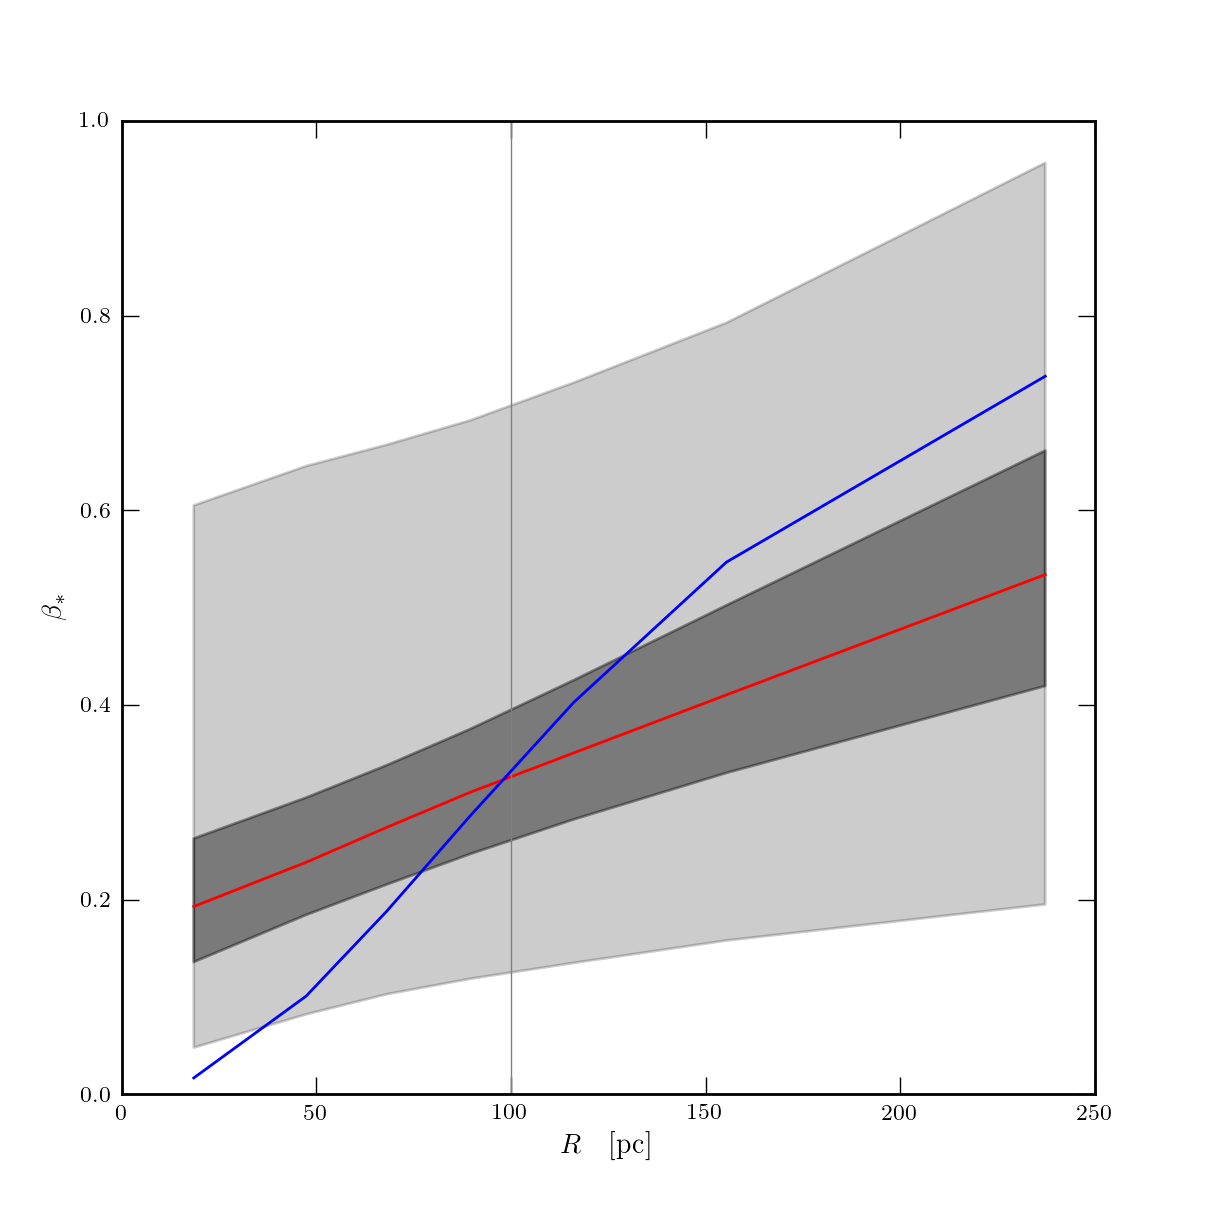
\includegraphics[width=0.3\textwidth]{fig/prof_betastar1.png}\TODO{generate fine plot again}

\caption{Reconstructed density and mass of a cusped model (red shows median,
  shaded areas are 68 and 90 percentiles) for $(2800,4033)$ tracer particles,
  after 50000 iterations. The black dashed curve shows the underlying
  theoretical model.}
\label{fig:cusp}
\end{center}
\end{figure*}

\TODO{d ln rho/d ln r, central density step}

% The errorbars around the scale radius of $1000$ pc of the dark matter
% cusp or the scale lengths of $500$ pc or $1000$ pc for the scale radii
% of the stellar components are not decreased, thus indicating that the
% relative values of the enclosed mass are not better constrained than
% at any other radius.


% nu and sigma: fit to data
Fitted $\nu(r)$ and $\siglos$ are shown in fig. \ref{fig:nusiglos}.

\begin{figure*}
\begin{center}
    \hspace{-7mm}
    \TODO{updated nu and sigma profiles with data in background}
    % 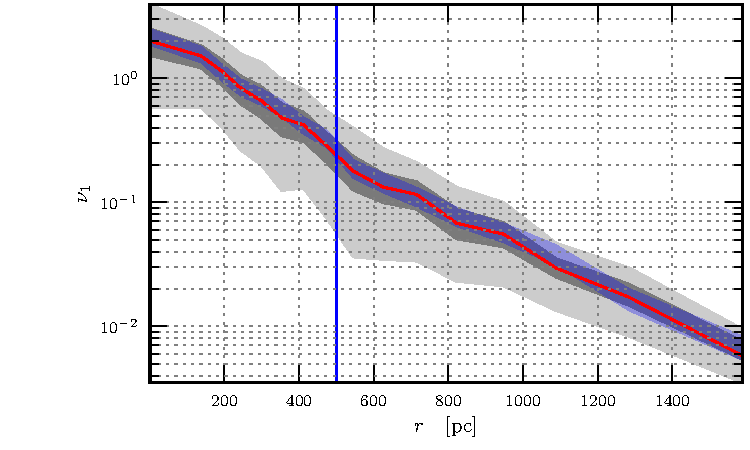
\includegraphics[width=0.5\textwidth]{fig/profnu1.pdf}
    % 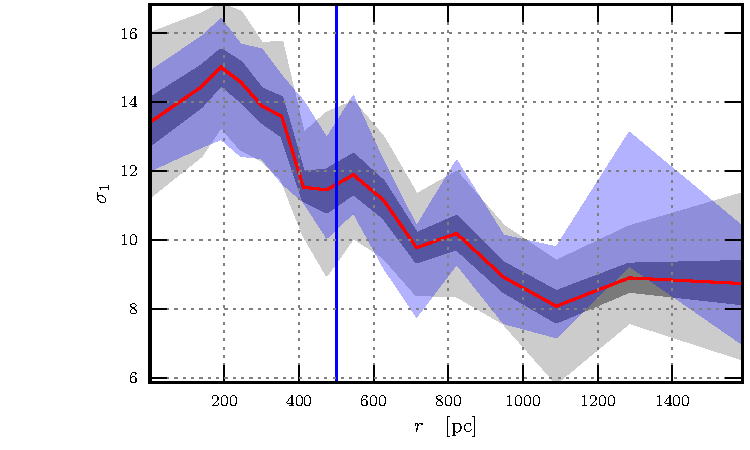
\includegraphics[width=0.5\textwidth]{fig/profsig1.pdf}
    \caption{\label{fig:nusiglos} Fitted $\nu(r)$ and $\siglos(r)$ for the
      first of two stellar components in the cusped profile of
      fig. \ref{fig:cusp}.}

\end{center}
\end{figure*}


% fit to underlying beta

The fitted $\beta_i(r)$ are shown in fig. \ref{fig:betai}.

\begin{figure*}
    \begin{center}
        \hspace{-7mm}
        \TODO{beta and betastar profile}
        %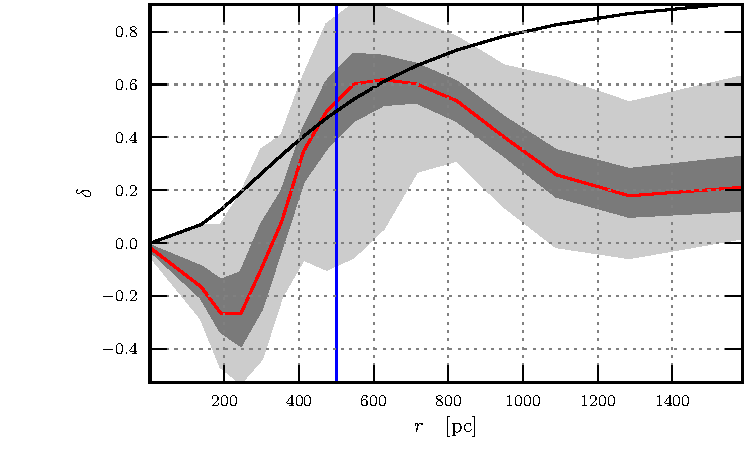
\includegraphics[width=0.5\textwidth]{fig/profdelta1.pdf}
        %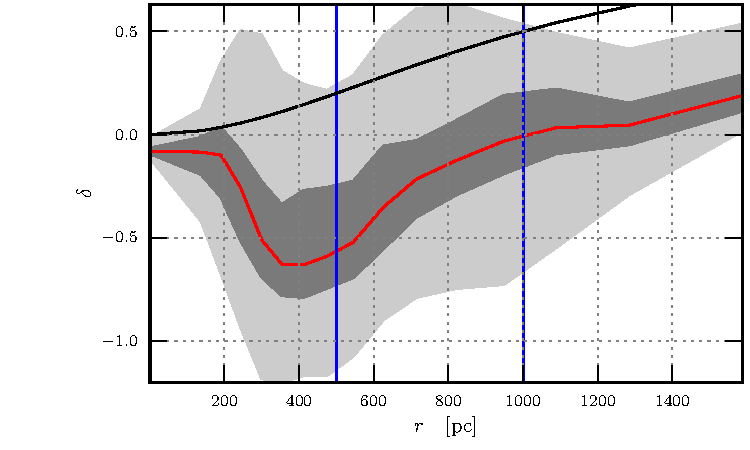
\includegraphics[width=0.5\textwidth]{fig/profdelta2.pdf}
        \caption{Fitted $\beta_i(r)$ for the two stellar components in the
          cusped profile of fig. \ref{fig:cusp}. The black line gives the
          $\beta$ profile of the underlying model. The horizontal lines are
          the 3D scale radii of the two stellar components.}
        \label{fig:betai}
    \end{center}
\end{figure*}



\begin{figure*}
    \begin{center}
        \hspace{-7mm}
        % TODO: generate kap1, kap2 files
        % \includegraphics[width=0.5\textwidth]{fig/profkap1.pdf}
        % \includegraphics[width=0.5\textwidth]{fig/profkap2.pdf}
        \caption{\label{fig:betai} Fitted $\kappa_i(r)$ for the two stellar
          components in the cusped profile of fig. \ref{fig:cusp}. The black
          line gives the $\kappa$ profile of the underlying model. The
          horizontal lines are the 3D scale radii of the two stellar
          components.}
    \end{center}
\end{figure*}

\TODO{observations for kurtosis}
\TODO{better/worse fitting of density}

Introducing $\kappa_i$ in the $\chi^2$ did \TODO{not?} result in a change of
behavior for the velocity anisotropy parameter. The mass was still
found too high, probably due to an error in projection of $\nu$ from
the modeled 3D density to a 2D surface density compared with data.


\subsection{Cored Model}
For a cored profile, we have a similar result, see fig. \ref{fig:core}. \TODO{rerun}

\begin{figure*}
    \begin{center}
        \hspace{-7mm}
        % \includegraphics[width=0.5\textwidth]{fig/.pdf}
        \caption{A cored profile: Reconstructed mass of the MCMC model (red
          shows median, shaded areas are 68 and 90 percentiles) for $10^4$
          tracer particles after 30000 iterations. The black dashed curve
          shows the underlying theoretical model.}
        \label{fig:core}
    \end{center}
\end{figure*}


\subsection{Triaxial mock data}
\TODO{motivation: triaxiality of observed dwarfs, effects from other
  mass modelling schemes}

The models were generated with a Made 2 Measure algorithm of
\cite{Dehnen2009} and are tailored to follow a similar profile to the
profiles specified above for the dwarf galaxies. They show a density
profile of

\begin{equation}
    \rho(r)=\frac{\rho_S}{\left(\frac{r}{r_S}\right)^\gamma\left(1+\left(\frac{r}{r_S}\right)^{1/\alpha}\right)^{\alpha(\beta-\gamma)}}
\end{equation}

with radius $r$, scale radius $r_S=1.5\kpc$, $\alpha=1$,
$\beta=4$. For the cusped profiles we have an inner logarithmic slope
of $-\gamma=-1$, scale density $\rho_S=5.522\cdot 10^7M_\odot/\kpc^3$,
and $M_{\tot}=1.171\cdot10^9M_\odot$, while for the cored one we have
$\gamma=0.23$, $\rho_S=1.177\cdot10^8M_\odot$,
$M_{\tot}=1.802\cdot10^9M_\odot$. The axis ratios are $b/a=0.8$ and
$c/a=0.6$. The stars have negligible mass and follow the same
functional form in the density profile as dark matter, with
$\alpha=0.34, \beta=5.92, \gamma=0.23, r_S=0.81\kpc$.

The velocity anisotropy of the stellar part is calculated via

\begin{equation}
\beta(r)=\frac{r_{s,\beta}^\eta \beta_0+r^\eta \beta_\infty}{r^\eta+r_{s,\beta}^\eta},
\end{equation}

with $r_{s,\beta}=0.81\kpc$, $\beta_0=0$, $\beta_\infty=0.5$ and
$\eta=0.5$, going from isotropic to radially anisotropic with
increasing radius.

\begin{figure*}
    \begin{center}
        \hspace{-7mm}
        \TODO{redo triaxial model}
        %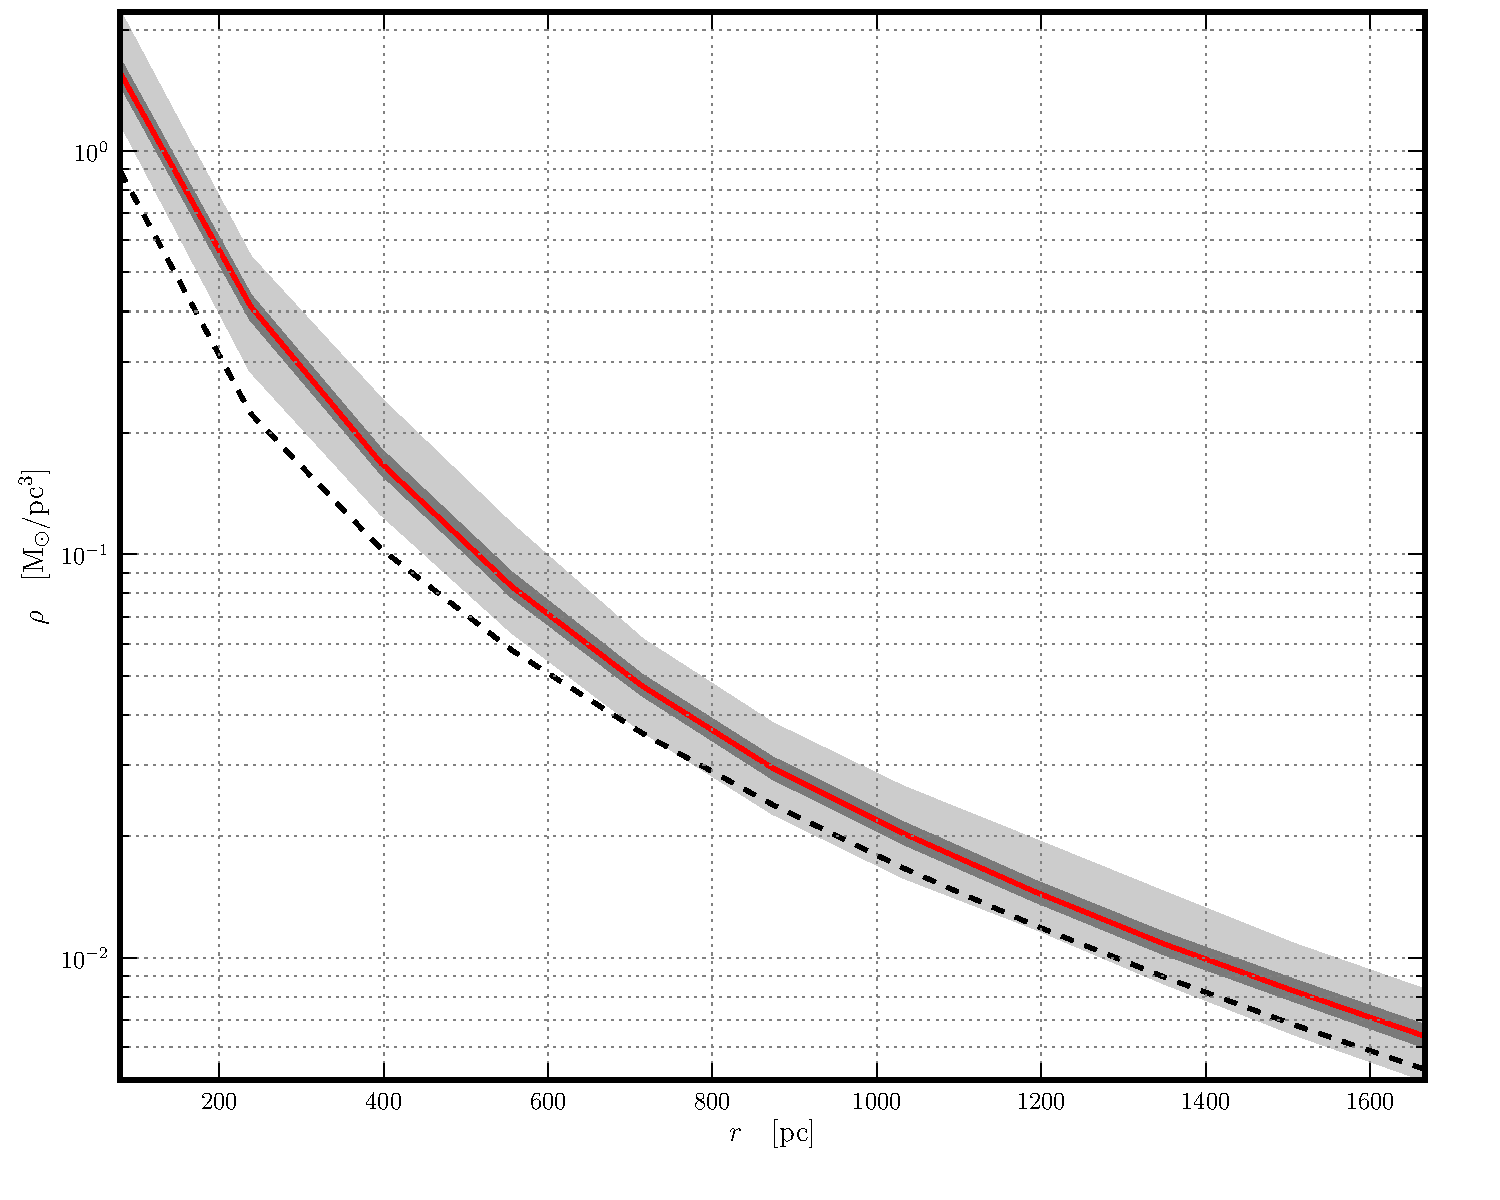
\includegraphics[width=0.5\textwidth]{fig/20130718123300_cprior_nulog_denslog_mslope_rprior_profdens.pdf}
        \caption{Density profile of a triaxial mock dwarf, for which the line
          of sight is inclined with 45 degrees with respect to all axes.}
        \label{fig:triax}
    \end{center}
\end{figure*}

The retrieved density profile (fig. \ref{fig:triax}) is constantly
overestimating the density.

\TODO{other projections}
\TODO{reason: projection}

